\section{Processor Architecture}

    \subsection{Y86 Instruction Set}
    In this instruction set some commands are split up into several.
        \begin{table}[ht]
            \centering
            \begin{tabular}{| l | l |}
                \hline
                halt   & stop the program\\
                \hline
                nop    & no operation\\
                \hline
                rrmovl & register $\to$ register\\
                \hline
                irmovl & immediate $\to$ register\\
                \hline
                rmmovl & register $\to$ memory\\
                \hline
                mrmovl & memory $\to$ register\\
                \hline
                OP1    & integer operation\\
                \hline
                jxx    & jumps\\
                \hline
                call   & call function\\
                \hline
                ret    & Return\\
                \hline
                pushl  & push onto stack\\
                \hline
                popl   & pop from stack\\
                \hline
            \end{tabular}
            \label{table:y86}
            \caption{Y86 Instruction Set}
        \end{table}

    \subsection{Sequential Implementations vs.\ Pipelining}
    In a sequential implementation, all cycles occur one after another. No new operation can start until the old one has finished.

        \begin{figure}[ht]
            \centering
            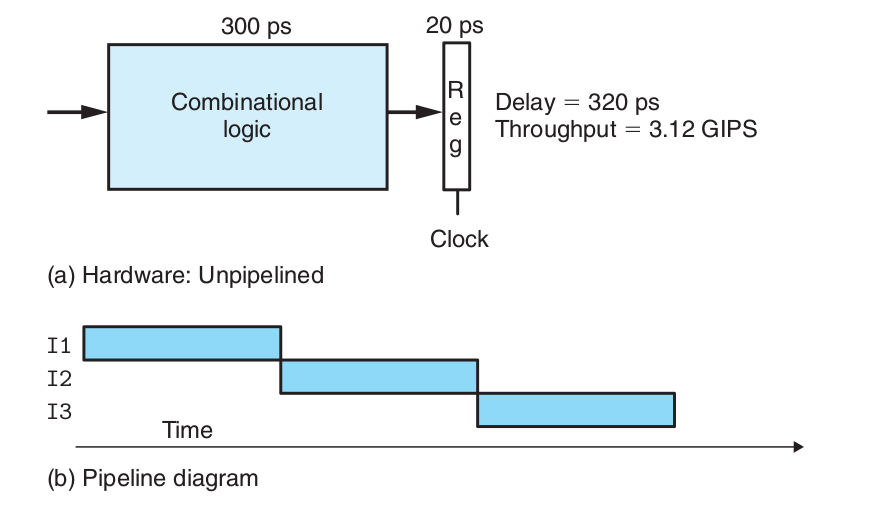
\includegraphics[scale=0.4]{./img/sequential.png}
            \caption{Sequential Implementation}
        \end{figure}

    Conversely in a pipelined implementation, we split up the cycles into stage and begin operations before old ones have finished.

        \begin{figure}[ht]
            \centering
            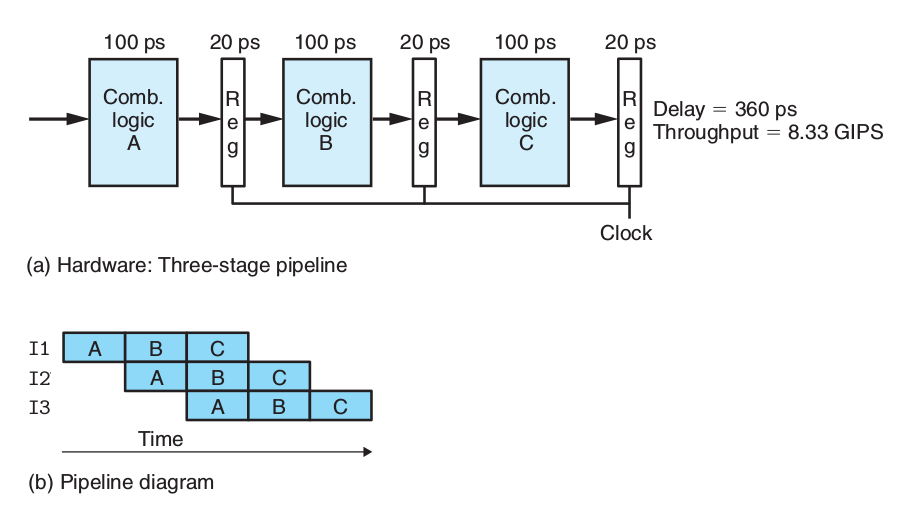
\includegraphics[scale=0.4]{./img/pipeline.png}
            \caption{Sequential Implementation}
        \end{figure}

\section{Optimization}
Optimization is an art.

We can use the metric \textit{cylces per element} (CPE) to express how effective a program is.

First step in code optimization is to reduce the number of bottlenecks. This is referred to as code motion.

After that's complete, we remove unnecessary memory referencing.

Follower by loop unrolling, the strategy that involves taking loops with a concrete number of steps and turning them into a set of similar commands.

Parallelization can be utilized in certain cases.

\section{Memory Hierarchy}

    \subsection{RAM}
    RAM comes in two forms, static and dynamic. Static RAM is much more expensive, but way faster.

        \subsubsection{SRAM}
        Each bit is stored in a bistable memory cell. It can only be in one position or another, never both, or neither. It will also keep its state indefinitely as long as it's kept powered.

        \subsubsection{DRAM}
        Each bit is stored as a charge on a capacitor. They lose power relatively quickly, and are much cheaper.

    \subsection{Disk Storage}
    Disks have several platters that spin at a fixed rate. The capacity of a disk is determined by

        \[ Recording \, Density \times Track \, Density = Areal \, Density \]

    or

        \[ Capacity = \frac{bytes}{sector} \times \frac{average sectors}{track} \times \frac{track}{surface} \times \frac{surfaces}{platter} \times \frac{platters}{disk} \]

    There is an actuator arm responsible for reading and writing from and to the disk.

    \subsection{Locality}
    There are two types of locality: Spatial and Temporal. Spatial locality refers to the fact that when memory is accessed, the memory around it is likely to be accessed in the near future. Temporal locality on the other hand refers to the notion that when memory is accessed, it's likely to be accessed again.

    \subsection{Memory Hierarchy}
    Each layer down in the memory hierarchy you go down, you slow the speed but decrease the cost. Therefore it's essential to introduce the concept of caching.

    Caching involves storing smaller chunks of memory in the fastest spots so that you can access them only when you need them. A cache hit occurs when the memory needed is in the cache. The memory is then used directly from there. Conversely, a cache miss occurs when the memory is not cached.

    Whenever there is a miss, the cache must use its replacement policy in order to determine which block to evict in order to make room for the new block.

        \subsubsection{Cache Capacity}
        The capacity of a cache can be expressed using the tuple $(S, E, B, m)$, where each memory address has $m$ bits, forming $M=2^m$ unique addresses, $S=2^s$ cache sets, $E$ cache lines, and $B=2^b$ data blocks. Caches also need $t=m-(b+s)$ tag bits that uniquely identify the cache line.

        Therefore capacity can be expressed as $C = S \times E \times B$

        \begin{figure}[ht]
            \centering
            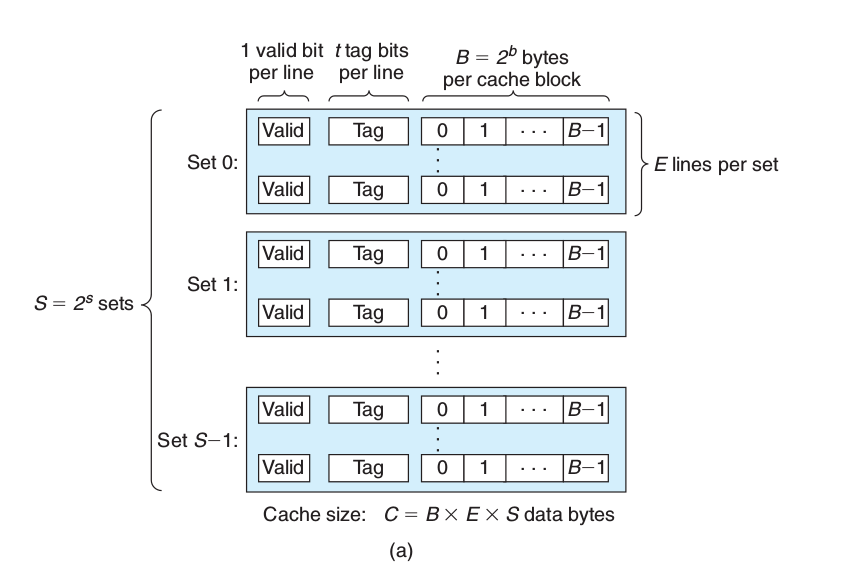
\includegraphics[scale=0.4]{./img/cache.png}
            \caption{Sequential Implementation}
        \end{figure}

        \subsubsection{Direct Mapped Caches}
        A cache with one line per set is a direct-mapped cache. When we have a cache miss, three steps occur.

        Step One: Set Selection. The correct set is located using $s$.

        Step Two: Line Matching. Determine if any line already contains the data. If one does, we have a cache hit.

        Step Three: Line Replacement. If we have a cache miss, we need to replace a line with the new data.

        \subsubsection{Set Associative Caches}
        Conflict misses arise when we have direct mapped caches, where there is one line per set. We can relax this constraint a little, and establish each set to have at least 2 lines. A set with $1 < E < C/B$ is called an $E$ way set associative cache. This is a much more sophisticated caching method, and we need to search each line separately instead of each set like before. The replacement policies differ from machine to machine, and it can be tricky determining what replacement method is utilized.

        \subsubsection{Fully Associative Caches}
        A fully associative cache has $E = C/B$. Set selection is trivial as there is only one set, however indexing is tricky given that there are many similar tags. These caches are not effective at a large scale.

